\chapter{黑洞可视化}
本章从经精度高、速度快和易用性强为出发点,实现了一个带有用户交互界面的黑洞图像离线渲染其,并对其性能进行了测试。
\section{模型的边界条件}
\begin{enumerate}
    \item 坐标系 \\ 史瓦西测地线的推导是建立在四维球坐标系$\left(t,r,\theta,\phi\right)$上。本程序不考虑时间膨胀,将坐标系简化为$\left(r,\theta,\phi\right)$。三维图形的绘制是建立在笛卡尔坐标系$\left(x,y,z\right)$上。程序使用右手定则确定笛卡尔坐标系,上方为y轴正半轴,右方为x轴正半轴,后方为z轴正半轴;
    \item 单位制 \\ 程序使用抽象长度与质量单位,避免使用米、千克、引力常数$G$、光速$c$等易造成浮点数溢出的大数。令$G=1$, $c=1$,质量单位为中心天体质量$M$,长度单位为$\nicefrac{GM}{c^2}=M$;
    \item 黑洞 \\ 程序中实现了一个不旋转不带电荷的史瓦西黑洞。黑洞奇点放置在世界坐标的原点$\left(0,0,0\right)$。史瓦西黑洞只具有一个性质:质量。黑洞的其他特征包括爱因斯坦环都由中心天体的质量和观测者的位置决定;
    \item 吸积盘 \\ 吸积盘是一个类似土星环围绕中心天体旋转的尘埃环状结构。黑洞拥有一个可选的圆形吸积盘,吸积盘是无限薄且不透明的。黑洞的吸积盘形态,但会有一些物理上的限制(例如吸积盘不会在光球以内)。吸积盘固定于黑洞位于世界坐标系中的赤道面上。宇宙中没有绝对的方向,调整相机的视角和天空盒的坐标就可以控制吸积盘的倾角;
    \item 天空盒 \\ 天空盒是一个正立方体,使用六张正方形图片描述从无限远处传来的光线。在这个程序中使用右手定则来确定天空盒的坐标,与世界坐标系一致。天空盒的采样坐标使用从世界原点出发的位置向量确定。天空盒使用像素天空盒,而不直接使用星表确定背景星空,是因为恒星与星系不是光线追踪的最小单位,光线才是。下图\ref{sub@fig:nasa-apod}是NASA每日一图(APOD)\cite{raytraceusingstarcatalogue}使用星表生成的黑洞示意图。原始背景为生成的大麦哲伦星云\ref{fig:lmc_apod}。\\ 注意背景恒星是圆形的,背景中黄色的尘埃物质在引力透镜下产生了形变。根据\ref{fig:camera_view_orbit}可以看出,光线在距离中心天体10M以上后受到引力的影像就很小了,可以将背景星体近似为无限远。真正所应看到的影像应该是类似\ref{sub@fig:nasa-apod-erratum},星光越接近黑洞视界越扭曲(作者网站上没有提供原始的完整的六面天空盒,红色部分是来自正面以外天空盒的光线)。
          \begin{figure}[H]
              \centering
              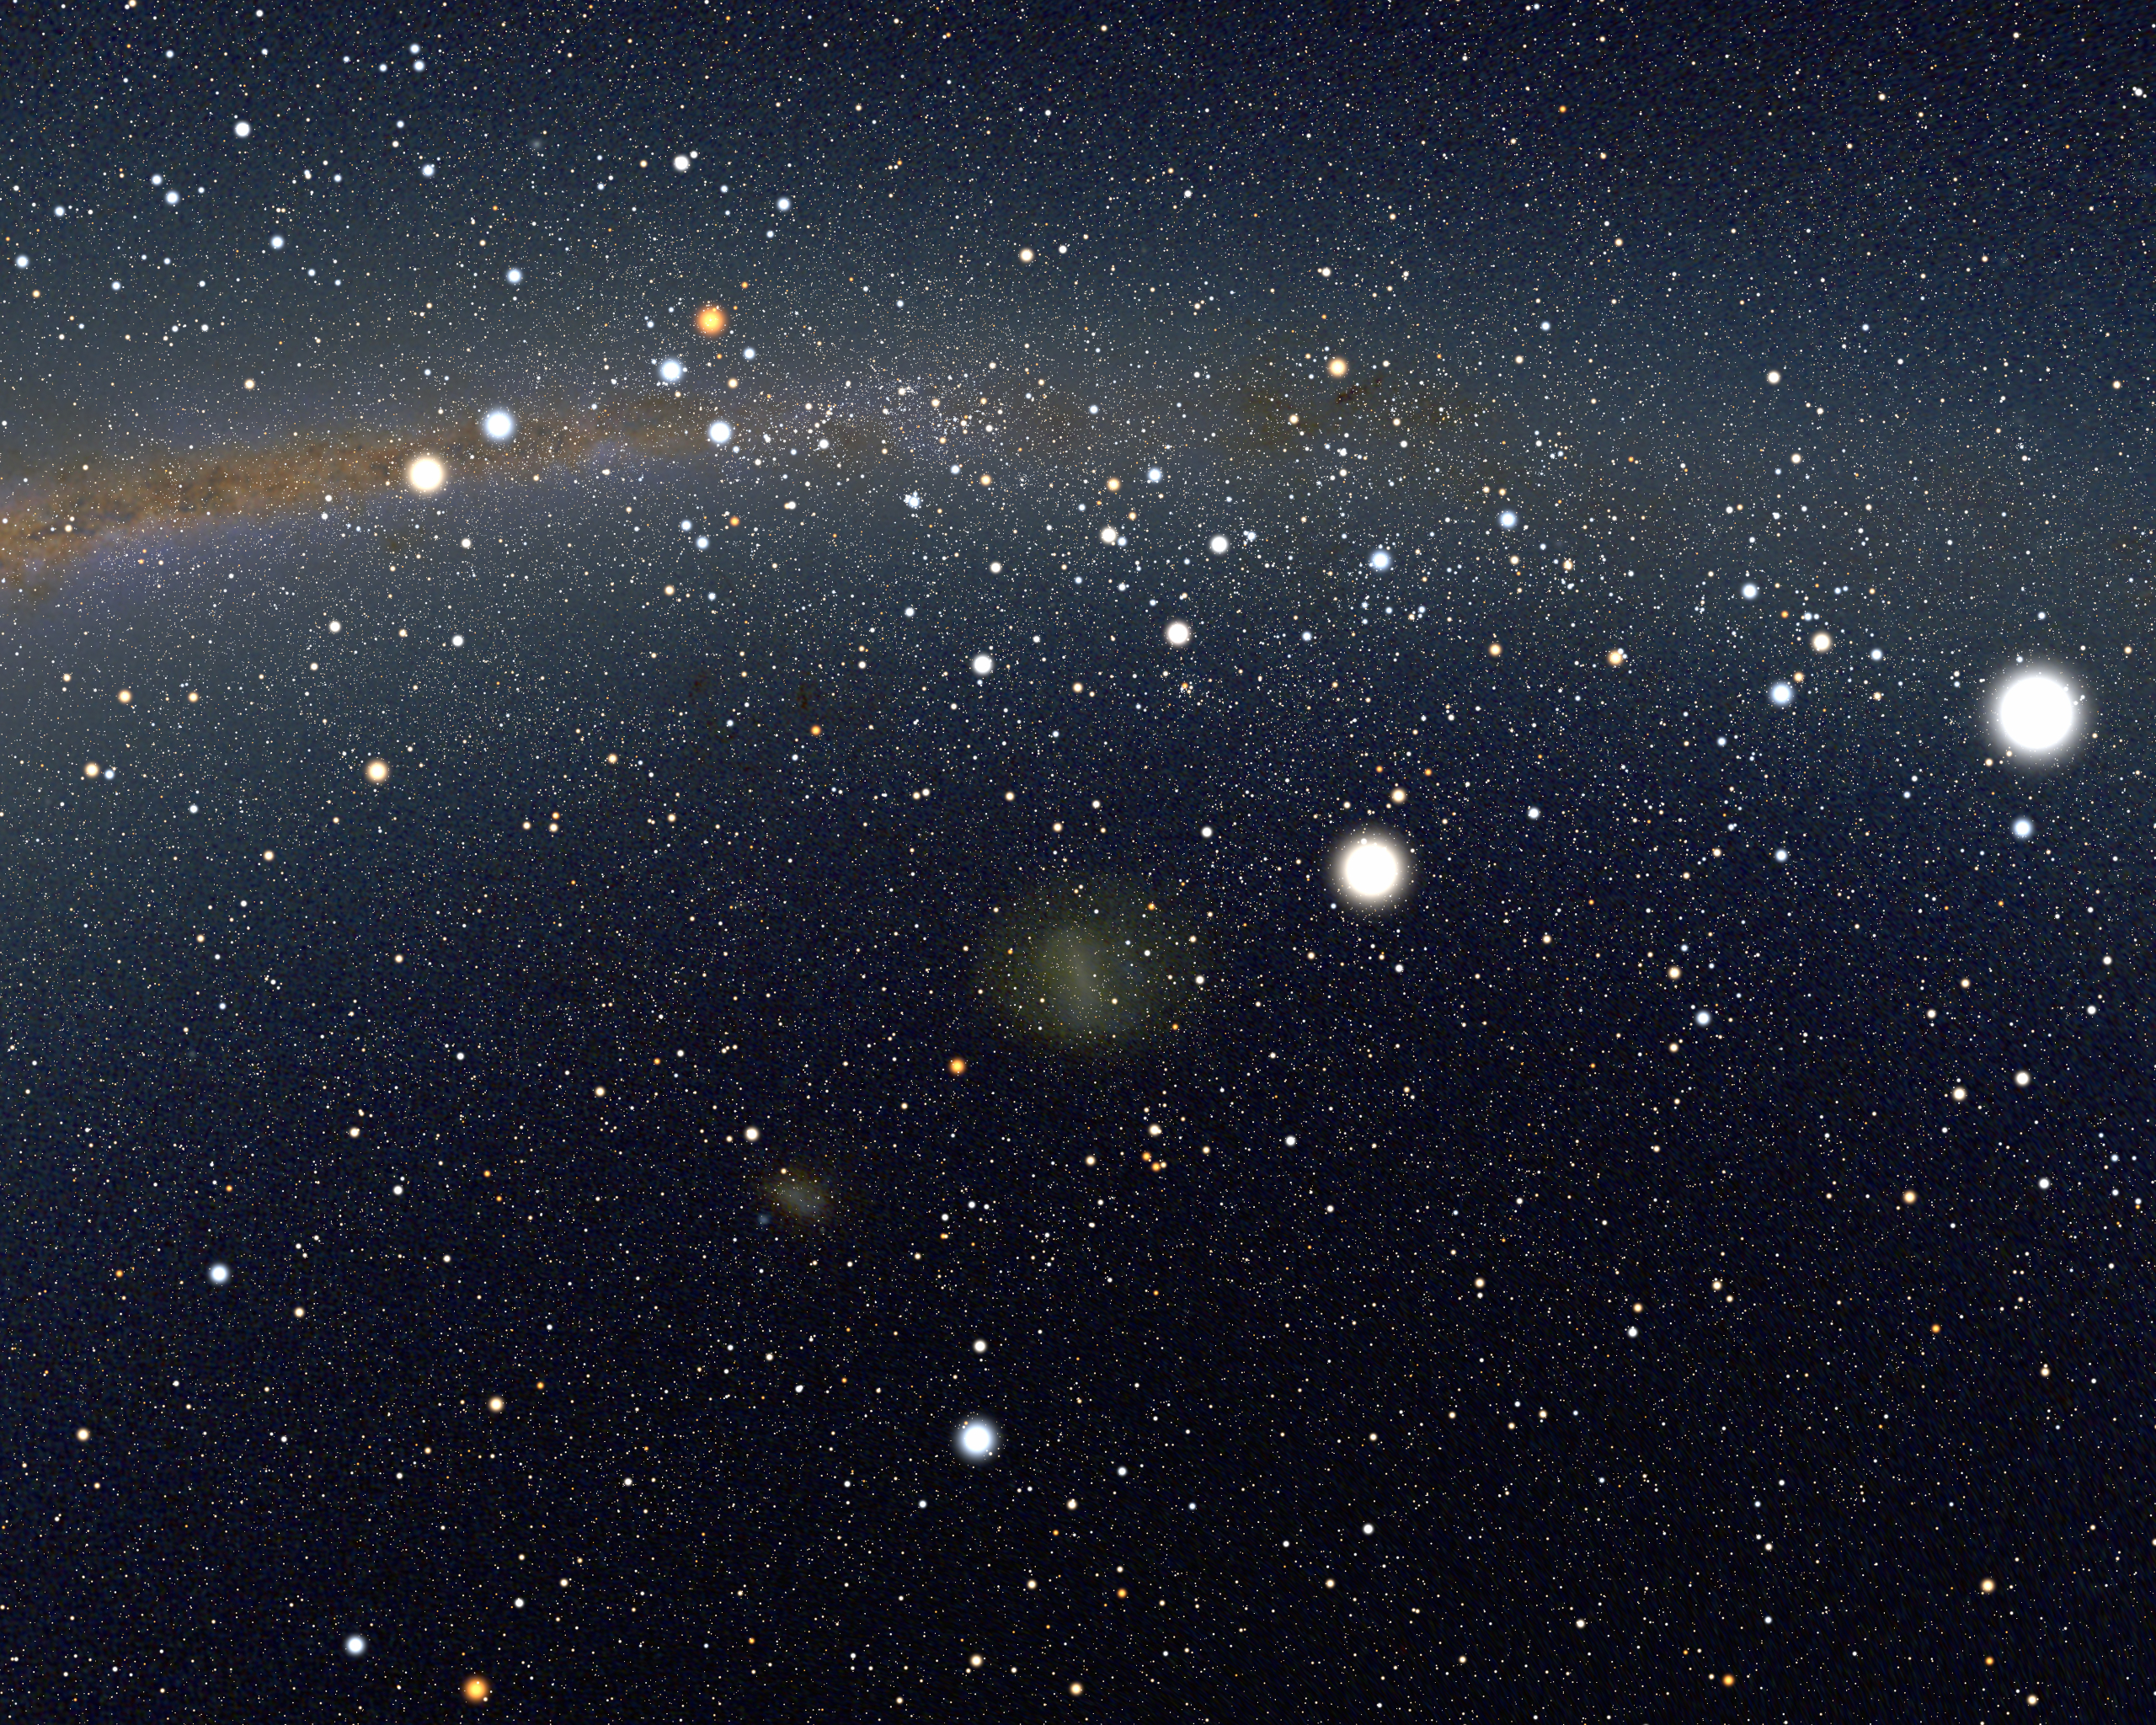
\includegraphics[scale=0.08]{images/LMC_APOD.jpg}
              \caption{原始背景(生成)}
              \label{fig:lmc_apod} % label 用来在文中索引
          \end{figure}
          \begin{figure}[htbp]
              \centering
              \begin{subfigure}{.5\textwidth}
                  \centering
                  \includegraphics[width=.8\linewidth]{images/bhlens_riazuelo.jpg}
                  \caption{NASA APOD 使用发光天体为单位进行追踪}
                  \label{fig:nasa-apod}
              \end{subfigure}%
              \begin{subfigure}{.5\textwidth}
                  \centering
                  \includegraphics[width=.8\linewidth]{images/bhlens_erratum.png}
                  \caption{使用像素为单位进行追踪}
                  \label{fig:nasa-apod-erratum}
              \end{subfigure}
              \caption{两种追溯星光的方法}
          \end{figure} 图\ref{fig:nasa-apod}应该是有意为之\cite{riazuelo_seeing_2018},但不应该是人眼所看到的影像。
    \item 相机 \\ 程序中拥有一个相机,相机有长宽比例、可视角度、世界坐标和观测角度等参数。以相机为中心,存在一个相机本地的坐标系,光子的发射角度由相机的参数,在相机本地坐标系下决定的。光线追踪需要一个本地坐标系到世界坐标系的转换。
\end{enumerate}


\section{离线渲染}
传统的光线追踪程序是通过判断光线(直线)与平面是否相交来判断光线是否击中物体的。近年随着消费级硬件性能提升,实时渲染领域光线追踪有取代光栅化的趋势。但也只是刚刚起步,只有最顶级的消费级显卡才能以Full HD画质在大多数游戏中实现令人满意的光线追踪渲染效果(60 FPS)。

黑洞附近的光线路径不再是直线,不能使用简单的直线求交方式判断光线的是否击中物体。每一束光线都要多次迭代才能获得光束的路径。

光线的追踪流程如下,撞击参数b依赖于发射角$\theta$,轨道近点$r_3$依赖于撞击参数b。光子的终点可能有三个:
\begin{enumerate}
    \item 击中吸积盘;
    \item 被吸入黑洞;
    \item 逃离黑洞到达无限远处。
\end{enumerate}
\begin{figure}[H]
    \centering
    \includegraphics[scale=0.75]{images/flowchart.pdf}
    \caption{单个像素光线追踪流程图}\label{fig:flowchart} % label 用来在文中索引
\end{figure}

\subsection{开发环境}
\begin{enumerate}
    \item 开发语言 \\ 开发语言主要用的是C++,在高性能计算方面,C++一直都是最好的选择。Rust的性能也很高,但是它有一个明显的缺点就是第三方库稀缺,诸如ffmpeg、OpenCV都没有很好的支持;
    \item 构建环境 \\ CMake是目前的项目构建环境,可以很好的满足跨平台构建的需求。这一点是MSBuild做不到的;
    \item 硬件环境 \\ CPU使用的是Intel Core i7-8750h,GPU是Nvidia RTX-2060。CPU有完整的AVX2指令集支持,GPU支持Vulkan API可以使用Compute Shader做通用计算;
    \item 图形界面框架 \\ 图形界面的框架选择的是QT5,跨平台的GUI框架没有太多的选择。
\end{enumerate}


\subsection{模型参数说明}
程序不需要输入黑洞的质量,因为长度单位与黑洞质量成正比,比例为$\nicefrac{G}{c^2}$。所需输入的参数有:
\begin{enumerate}
    \item 吸积盘的几何与纹理 \\ 吸积盘是一个圆环,需要设定吸积盘的内径与外径。还需要输入吸积盘的纹理图片,可以使用一维纹理也可以使用二维纹理;
    \item 天空盒纹理 \\ 天空盒是六张分别代表上、下、左、右、前、后的正方形纹理图片,也可以是使用六面图层的一张图片,还可以使用六张拼接成一张的天空盒立方展开图;
    \item 相机设定 \\ 唯一需要输入的坐标是相机的世界坐标,还需要相机本地坐标系中三个轴其中的两个在世界坐标系中的方向向量,知道其中两个可以计算第三个,用于确定相机的方向。相机x轴与y轴分别有一个视场(FoV)设定,用于确定光子发射角的最大值。
\end{enumerate}


\subsection{光线追踪的实现}
跟其他传统的光线追踪方法一样,光线是逆向追踪,从相机的坐标出发,这能极大的减轻运算量,但会导致采样的图片有噪点或者信息缺失,这个会通过多重采样来缓解。

三维坐标系跟二维坐标系下的光线追踪方法是类似的。根据史瓦西时空的对称性,需要确定一个光线偏转轴,然后根据这个偏转轴确定光子在测地线积分路径上的坐标。

每一束光线都有它偏折时对应的偏转轴。光子的偏转轴确定为光子发射时的速度向量与相机位置向量的叉乘。实现向量的旋转可以选择在极坐标系也可以选择在笛卡尔角坐标系下进行。选择在笛卡尔坐标系下进行向量旋转。这样可以利用已知的欧拉角旋转矩阵简单的对向量进行旋转。

\paragraph{没有吸积盘的情况}
在黑洞没有吸积盘的情况下,只需要根据之前的推出的结论以光线的初始条件撞击参数b,确定光线是否会坠入黑洞。如果光线坠入黑洞,像素点的采样就是黑色的。如果光线没有坠入黑洞,则需要选定一个光线的积分终点,近似为光线传播到无限远处时的积分终点。如果直接求无限积分,就需要一套复杂的数值计算系统,其实是没有必要的。因为根据上面的结论,光线在距离黑洞20M以上之后就基本上不会受到空间弯曲的影响了。

将近似无限远处的积分终点$r_1$设为2000M,这个范围完全足够了。整个测地线积分分为两段,从相机原点$r_0$到光线近点$r_3$,再从光线近点$r_3$到设定的积分终点$r_1$。其中有一段重复的积分范围,从$r_0$到$r_3$再从$r_3$到$r_0$,这两段互为相反数,实际积分的时候可以省掉重复的一段。

对测地线积分的结果为光线在一个极坐标平面上极角的变化量。也就是在三维坐标系中,光子对于偏转轴所要偏转的角度。可以使用旋转矩阵\cite{rotation_matrix}绕轴$\vec{u}=\left(u_x,u_y,u_z\right)$旋转$\theta$度
\begin{equation}
    \begin{bmatrix}\cos\theta+u_{x}^{2}\left(1-\cos\theta\right)       & u_{x}u_{y}\left(1-\cos\theta\right)-u_{z}\sin\theta & u_{x}u_{z}\left(1-\cos\theta\right)+u_{y}\sin\theta \\
        u_{y}u_{z}\left(1-\cos\theta\right)+u_{z}\sin\theta & \cos\theta+u_{y}^{2}\left(1-\cos\theta\right)       & u_{y}u_{z}\left(1-\cos\theta\right)-u_{x}\sin\theta \\
        u_{z}u_{x}\left(1-\cos\theta\right)-u_{y}\sin\theta & u_{z}u_{y}\left(1-\cos\theta\right)+u_{x}\sin\theta & \cos\theta+u_{z}^{2}\left(1-\cos\theta\right)
    \end{bmatrix}
\end{equation}

旋转完后就能得到光子在$r_1$的位置向量,实际上近似于光子在$r_1$的速度向量,也是最终在天空盒上采样的方向向量。

\paragraph{有吸积盘的情况}
黑洞如果拥有吸积盘,上面两种情况的光线都有可能与吸积盘相交。

首先可以通过计算光子轨道近点排除完全不可能与吸积盘相交的光子,也就是光子不会进入由吸积盘圆环内圆与外圆所在的同心球壳之间的空间,光子会直接射向无限远处的天空盒。

如果光线进入吸积盘同心球壳,存在三种情况:

\begin{itemize}
    \item 光子近点在吸积盘范围内,需要从外径积分到近点再积分到外径
    \item 光子近点在吸积盘内径以内,最终坠入黑洞,
    \item 光子近点在吸积盘内径以内,则从吸积盘外径积分到内径
\end{itemize}

判断吸积盘与光子相交,通过判断光子在吸积盘范围(吸积盘外径所在球壳与内径所在球壳之间的空间)内是否穿过赤道面。有两个充分条件(sufficient condition)可以判断:
\begin{enumerate}
    \item 光子在吸积盘范围内的运动极角变化大于$\ang{180}$,因为光子绕中心天体运动,极角变化超过$\ang{180}$必定与赤道面相交;
    \item 光子在吸积盘范围内运动的起始坐标与终止坐标的y轴部分符号不同。
\end{enumerate}

当其中一条满足就要进入光线与吸积盘相交的采样过程,这个过程是整个渲染中最消耗CPU时间的部分。

可以选择数值求解的方法得到光子进入吸积盘范围后达到吸积盘所需要的偏转角度,也可以通过逐步模拟的方法对光线进行追踪,本设计选择后者。为了提高速度,选择了可变步长的逐步追踪,当光子越接近赤道面时,步长越小,这样能有效减少迭代次数。最终光线与吸积盘相交时的坐标就可以转换为吸积盘纹理的采样坐标。

\subsection{图像处理}

\begin{enumerate}
    \item 纹理采样 \\ 程序中需要用到纹理采样的地方有两个,天空盒与吸积盘。天空盒的采样只需要一个光线的速度向量,在六面天空盒上对应采集纹素。吸积盘的纹理横轴均匀分布在吸积盘的一周,纵轴则是从外径到内径。吸积盘的采样需要光子打在吸积盘上的绝对坐标(赤道面上的二维坐标),转换为极坐标后就是纹素的二维坐标;
    \item 抗锯齿 \\ 程序的抗锯齿是一个简单的MSAA (Multisample Anti-Aliasing)抗锯齿,这个过程发生在光子从相机出发的时候,而不是对天空盒和吸积盘采样的时候,因为黑洞本身也需要抗锯齿,不只是纹理。\\ 抗锯齿的采样点选取是一个简单的均匀分布随机采样,给光子的发射时的速度向量增加一个与分辨率成反比的摄动(perturbation)。将多个光线追踪后的采样值叠加得到最后的单个像素颜色;
    \item 后处理 \\ 程序有一个图像后处理功能,是给吸积盘加上bloom的效果。为了做到这个,需要一个光源缓冲区记录吸积盘本身,因为只有吸积盘是发光的。将光源缓冲区进行高斯模糊,得到吸积盘的bloom效果。将光源缓冲区与原始的颜色缓冲区叠加后得到一张HDR图片,对HDR图片进行Tone Map和伽马矫正后得到最终的显示图像。
          \begin{figure}[H]
              \centering
              \begin{subfigure}{.5\textwidth}
                  \centering
                  \includegraphics[width=.8\linewidth]{images/no-bloom.png}
                  \caption{未处理图像}
                  \label{fig:no-bloom}
              \end{subfigure}%
              \begin{subfigure}{.5\textwidth}
                  \centering
                  \includegraphics[width=.8\linewidth]{images/bloom.png}
                  \caption{blooming后的图像}
                  \label{fig:bloomed}
              \end{subfigure}
              \caption{bloom效果}
          \end{figure}
\end{enumerate}

\subsection{用户图形界面设计}
用QT框架给程序包裹了一层图形界面,方便使用。程序的前端图形界面与后端渲染引擎是分离的,引擎完全不依赖图形界面,使用命令行也可以实现其功能。
\begin{figure}[H]
    \centering
    \includegraphics[scale=0.5]{images/gui.png}
    \caption{程序界面}
    \label{fig:gui} % label 用来在文中索引
\end{figure}
窗体的左侧是渲染状态,可是实时预览渲染的情况,这样就省去了进度条的显示。右侧是程序输入与设定,基本上涵盖了渲染所需要设定的参数与纹理。图片渲染完成后可以保存到硬盘上。


\subsection{成像效果}

\subsubsection{天空盒成像}
首先使用这个方格棋盘背景作为天空盒来演示光线偏折的效果,每一面的天空都是一样的
\begin{figure}[H]
    \centering
    \begin{subfigure}{.5\textwidth}
        \centering
        \includegraphics[scale=0.2]{images/chessboard.png}
        \caption{棋盘天空盒,没有黑洞的时候看到的背景}
        \label{fig:chessboard} % label 用来在文中索引
    \end{subfigure}%
    \begin{subfigure}{.5\textwidth}
        \centering
        \includegraphics[scale=0.2]{images/blackhole_chessboard.png}
        \caption{距离黑洞100M}
        \label{fig:blackhole-chessboard} % label 用来在文中索引
    \end{subfigure}
    \caption{在场景中有无黑洞的对比}
\end{figure}

光线越接近黑洞,产生的偏折越大,当光线靠近光子轨道$r=3M$处时,光子会开始短暂环绕黑洞\ref{fig:camera_view_orbit},光线会来自天空盒的各个面,所以黑洞附近的图像方格非常密集。

使用一个\ang{360}全景图作为天空盒可以从另一个角度直观感受光线的偏折,
\begin{figure}[H]
    \centering
    \begin{subfigure}{.5\textwidth}
        \centering
        \includegraphics[width=.8\linewidth]{images/building.png}
        \caption{天空盒的一面}
        \label{fig:building}
    \end{subfigure}%
    \begin{subfigure}{.5\textwidth}
        \centering
        \includegraphics[width=.8\linewidth]{images/building_distort.png}
        \caption{变形后的图像}
        \label{fig:building_distort}
    \end{subfigure}
    \caption{在世界中心添加一个黑洞}
\end{figure}
从这个发生形变的图像可以看出一些黑洞附近光线轨迹的特点:
\begin{enumerate}
    \item 两旁的树有可见的像有两个,一个是树的主像,在图像的两侧,在接近黑洞中心的位置有一个倒立的次级像。这很像凸透镜的效果;
    \item 房子二楼的栅格围栏刚好在黑洞的后面,整个围栏的产生巨大的形变,但围栏是完整的,信息并没有丢失;
    \item 围栏形成了一个环状结构,其实是最外层的爱因斯坦环;
    \item 接近黑洞视界下面的部分有一束白光,这束白光是变形后被拉长的太阳,在天空盒的背面,这是黑洞引力透镜成像与凸透镜不一样的地方。
\end{enumerate}
如果将图\ref{sub@fig:building_distort}放大,在靠近黑洞视界的地方可以清楚的看到后方的太阳。这是太阳的次级像(二次像)(主像并没有在图片中展示出来,但并不等于没有。太阳的主像来自摄像机的背后,只要摄像机的视场够大就能看到主像)。

\begin{figure}[H]
    \centering
    \begin{subfigure}{.33\textwidth}
        \centering
        \includegraphics[width=.95\linewidth]{images/zoomin_6x.png}
        \caption{放大6倍}
        \label{fig:zoomin-6x} % label 用来在文中索引
    \end{subfigure}%
    \begin{subfigure}{.33\textwidth}
        \centering
        \includegraphics[width=.95\linewidth]{images/zoomin_60x.png}
        \caption{放大60倍}
        \label{fig:zoomin-60x} % label 用来在文中索引
    \end{subfigure}
    \begin{subfigure}{.33\textwidth}
        \centering
        \includegraphics[width=.95\linewidth]{images/zoomin_600x.png}
        \caption{放大600倍}
        \label{fig:zoomin-600x}
    \end{subfigure}%
    \caption{第二个爱因斯坦环}
\end{figure}


如果再放大\ref{fig:zoomin-6x}的右上角的视界部分得到\ref{fig:zoomin-60x},可以看到后方太阳的三次像,这是第二个爱因斯坦环。

\begin{figure}[H]
    \centering
    \begin{subfigure}{.45\textwidth}
        \centering
        \includegraphics[width=.8\linewidth]{images/zoomin_6000x.png}
        \caption{放大6000倍}
        \label{fig:zoomin-6000x}
    \end{subfigure}
    \begin{subfigure}{.45\textwidth}
        \centering
        \includegraphics[width=.8\linewidth]{images/zoomin_60000x.png}
        \caption{放大60000倍}
        \label{fig:zoomin-60000x}
    \end{subfigure}
    \caption{第三个爱因斯坦环}
\end{figure}

将\ref{fig:building_distort}放大60000倍,这是太阳的四次像,第三个爱因斯坦环。四次像说明这束光线环绕黑洞转了两圈半。注意到图\ref{fig:zoomin-60x}与图\ref{fig:zoomin-60000x}是非常相似的两张图片,这意味着黑洞边界的图像是可以无限细分的。光线每围绕黑洞转一圈,就会在靠近黑洞视界的形成一个完整的世界的像。

爱因斯坦环是指星星的主像与次级像对称地成像在黑洞的两侧,两侧光线剧烈扭曲而形成的一个环状结构。爱因斯坦环太空中会比较明显,因为背景是黑色的,会显示为一个黑洞周围的亮环。
\begin{figure}[H]
    \centering
    \begin{subfigure}{.5\textwidth}
        \centering
        \includegraphics[width=.8\linewidth]{images/no_ring.png}
        \caption{背景星空}
        \label{fig:no-ring}
    \end{subfigure}%
    \begin{subfigure}{.5\textwidth}
        \centering
        \includegraphics[width=.8\linewidth]{images/einstein_ring.png}
        \caption{距离黑洞64M}
        \label{fig:einstein-ring}
    \end{subfigure}
    \caption{背景中心光线被扭曲成环}
\end{figure}
图中中心的光线被分散到黑洞的四周,形成一个光环。

\subsubsection{吸积盘成像}
出于直观考虑,制作了一个方格型的吸积盘贴图,吸积盘设定是一个无线薄的圆环,原则上从侧面看吸积盘是看不到的,将贴图的首尾相连形成一个环状就是吸积盘的外观。
\begin{figure}[H]
    \centering
    \includegraphics[scale=0.5]{images/flag.png}
    \caption{吸积盘贴图}
    \label{fig:disk-flag-texutre} % label 用来在文中索引
\end{figure}
从正上方观察黑洞会看到吸积盘是一个正圆环,光线会被黑洞拉向中心(吸积盘观察到的内径与外径相比实际的内外径偏小),
\begin{figure}[H]
    \centering
    \begin{subfigure}{.5\textwidth}
        \centering
        \includegraphics[width=.8\linewidth]{images/disk_top.png}
        \caption{上方观察黑洞与吸积盘}
        \label{fig:disk_top}
    \end{subfigure}%
    \begin{subfigure}{.5\textwidth}
        \centering
        \includegraphics[width=.8\linewidth]{images/equatorial_plane.png}
        \caption{在赤道面观察}
        \label{fig:einstein-ring}
    \end{subfigure}
    \caption{正对吸积盘观察}
\end{figure}
在赤道面上观察,可以看到背面的吸积盘所成的两个对称像。

在赤道面上方一点点,可以观察到黑洞正面吸积盘的主像与背面的主像(上方半圆)衔接,而背面的次级像(下方半圆)与处在黑洞视界边缘的黑洞正面吸积盘的次级像衔接(下方半圆在赤道上迅速缩小到黑洞视界边缘)。
\begin{figure}[H]
    \centering
    \begin{subfigure}{.5\textwidth}
        \centering
        \includegraphics[width=.8\linewidth]{images/above_equatorial_plane.png}
        \caption{上方观察黑洞与吸积盘}
        \label{fig:above_equatorial_plane}
    \end{subfigure}%
    \begin{subfigure}{.5\textwidth}
        \centering
        \includegraphics[width=.8\linewidth]{images/stand_on_disk.png}
        \caption{相机在吸积盘上观察}
        \label{fig:einstein-ring}
    \end{subfigure}
    \caption{视角与吸积盘倾斜时观察}
\end{figure}

\subsection{动态模拟}
动态的模拟可以更直观的看到,运动的相机是如何感知黑洞周围的光线的,或者演示旋转的吸积盘是如何被黑洞引力拉扯的。

程序有一个生成视频的接口,使用的是ffmpeg的C++库。用户需要输入每一帧相机的坐标与方向数据到文件里,使用接口读入文件就可以生成视频文件了。视频编码需要的是每一帧的图像数据,本设计是用的是8比特3通道图像,每一帧的生成都可以在GUI中预览,每一帧渲染完成后,将图像使用VP9编码,最后一帧生成后,将编码后的视频放进MP4容器中存入硬盘。

\section{性能测试}
\subsection{CPU与GPU性能}
一般而言,GPU在并行计算上相对于CPU有非常大的优势,特别是这种以像素为单位的渲染。
\subsubsection{CPU性能优化}
\begin{enumerate}
    \item 多线程 \\ 尝试过使用OpenMP实现多线程加速,使用OpenMP的Dynamic调度器性能并不是最佳的,不如手动调度用户线程。使用C++原子类型给每一个渲染块加锁,分配到不同的线程上,可以保证渲染过程中CPU利用率可以达到95\%以上,相比之下Python的多线程原型只能利用CPU所有核心的80\%左右;
    \item SSE/AVX2 \\ 一些像素操作使用AVX2指令集进行了优化,但是程序最耗时的部分并不是浮点数操作,而是积分计算;
    \item 积分方法 \\ 对测地线的积分是整个程序的核心,积分的精度决定了产出图像的质量,积分的速度决定了渲染的时间。在CPU渲染中使用了GNU Scientific Library中的数值积分方法,实际上是一个Fortran的QUADPACK算法,在Python中进行原型设计的时候scipy的积分方法也是对Fortran的QUADPACK二进制库的链接。QUADPACK是一个比较可靠的积分算法,一般情况下精度与速度都是在可接受范围内。
\end{enumerate}

\subsubsection{GPU性能优化}
尝试完全使用GPU进行渲染,框架选择为Vulkan API中的Compute Shader。之所以没有选择CUDA是因为Vulkan API是cross-vendor的。整个渲染过程使用双精度浮点保证渲染质量。

GLSL里没有科学计算库,函数数值积分的功能只能自己实现。尝试写了几个积分函数包括:
\begin{itemize}
    \item Runge-Kutta 4th order (RK4)
    \item Matlab中的ode23\cite{ode23}
    \item Runge-Kutta-Fehlberg Method (RKF45)\cite{numerical_methods_matlab}
\end{itemize}
它们的积分精度是递增的。因为测地线函数在一定范围内是一个单调函数,比较复杂的RKF45其实是不太适合,应为要多次计算测地线函数,导致它的速度比较慢。ode23速度很快,甚至很多情况比QUADPACK还快,精度也不错。

尝试使用Vulkan API的Compute Shader利用GPU进行并行计算。积分方法使用ode23,其速度在CPU上測試与CPU渲染器使用的QUADPACK算法是一个数量级的。在一个场景测试下,CPU使用16线程,GPU 线程 group size $32\times32$, dispatch $256\times256$ groups,得到如下性能数据
\begin{table}[H]
    \linespread{1.5}
    \zihao{5}
    \centering
    \caption{GPU与CPU渲染对比表,分辨率$512\times512$}
    \begin{tabular}{*{5}{>{\centering\arraybackslash}p{5cm}}}
        \hline
        CPU (quadpack) & GPU (ode23) \\ \hline
        6339ms         & 13098ms     \\ \hline
    \end{tabular}
\end{table}
而且GPU平均功耗在80瓦左右,CPU满载功耗只有45瓦。可能的原因在上面已经提到了。事实上电影《星际穿越》的黑洞渲染器也是纯CPU渲染的\cite{james_gravitational_2015}。GPU做高精度数值计算是不合适的。

在这种高精度渲染的目的下,GPU并不能胜任,可能有几点原因:
\begin{enumerate}
    \item GPU主频不高仅有1500 Mhz左右,不擅长循环次数多的算法;
    \item 高精度迭代追踪需要双精度浮点,甚至128位浮点数。根据英伟达图灵架构白皮书\cite{nvidia-turing-architecture-whitepaper}本世代GPU只有非常小的核心面积是用于双精度浮点数计算的,速度只有32位浮点数的\nicefrac{1}{32};
    \item 内存扩展性,最好的显卡内存不到30G,CPU内存可以轻松超过这个大小。虽然可以用tile-based rendering解决这个问题,但远不如CPU扩展方便。像上述可以放大60000倍的图片,很难在GPU中保存。
\end{enumerate}

\subsection{与starless性能对比}
尽量使用同一渲染设定来对比本设计与starless渲染器的效果与性能。设定如下:
\begin{itemize}
    \item 相机位置$(0, 1, 10)$;
    \item 分辨率$1024\times1024$;
    \item 渲染线程数16。
\end{itemize}
图片均为未经后处理的原始渲染结果,
\begin{figure}[H]
    \centering
    \begin{subfigure}{.5\textwidth}
        \centering
        \includegraphics[width=.8\linewidth]{images/starless_test.png}
        \caption{starless渲染的图片}
        \label{fig:starless_test}
    \end{subfigure}%
    \begin{subfigure}{.5\textwidth}
        \centering
        \includegraphics[width=.8\linewidth]{images/blackness_test.png}
        \caption{本设计渲染的图片}
        \label{fig:blackness_test}
    \end{subfigure}
    \caption{生成图片对比}
\end{figure}

\begin{table}[H]
    \linespread{1.5}
    \zihao{5}
    \centering
    \caption{starless与本设计渲染时间对比表,分辨率$1024\times1024$}
    \begin{tabular}{*{5}{>{\centering\arraybackslash}p{5cm}}}
        \hline
        starless & 本设计 \\ \hline
        41s      & 1.2s   \\ \hline
    \end{tabular}
\end{table}



\subsection{离线渲染与实时渲染}
本文侧重点是离线渲染,在上述利用GPU渲染比CPU还慢的情况下,使用这个算法进行实时渲染已经不可能了。但是可以用一个近似公式达到一个相似的效果。当相机距离黑洞较远的时候,光子测地线方程\ref{eq:geodesic}会简化成
\begin{equation}
    \Delta\theta\approx\frac{4M}{b}
\end{equation}
其中$\theta$为光线相对于光线出发时所在直线的偏转角度,撞击参数b会被简化为光线出发时所在直线与黑洞中心的垂直距离。

在OpenGL中实现这个光线偏折方程得到下面的结果,可以稳定60FPS渲染,
\begin{figure}[H]
    \centering
    \includegraphics[scale=0.5]{images/realtime.png}
    \caption{OpenGL实时渲染效果}
    \label{fig:realtime} % label 用来在文中索引
\end{figure}

这个算法有如下缺点:
\begin{enumerate}
    \item 最多只能看到物体的两个像,即一个爱因斯坦环可见;
    \item 近距离观察黑洞,光线的追踪是不准确的。
\end{enumerate}

